\chapter{Introduction}

\label{intro}

\dropcap{A}{ccurate}, efficient and high-resolution methods of surface water detection are needed to develop a better water management policy, provide input for hydrological and hydraulic models, and to deal with a plethora of satellite information becoming available for a steadily growing number of users. Monitoring of surface water extent and dynamics is essential for a better understanding of natural processes, anthropogenic factors as well as climate changes. 

Recent international agendas on climate change and environment demand objective information on planetary land and water surface conditions and changes, to be able to study the drivers behind them. The UN Sustainable Development Goals (GSDs) define seventeen challenges to be achieved by 2030, and almost half of them will directly or indirectly require up to date and high-resolution information on surface water. To name some, sustainable management of water and its use for food production, the role of the surface water for the spreading of deceases, climate change, and many other. 

The Intergovernmental Panel on Climate Change (IPCC) in the Technical Paper VI on Climate Change and Water defines knowledge gaps in observations and our understanding of the behavior of water. Moreover, with the variety and volumes of Earth Observation (EO) data available today, these gaps frequently mean the lack of proper algorithms to process existing data. The raw data need to be processed properly to derive higher level variables easily interpretable by broader, frequently non-academic, community. 

\section{Research Questions}

Many attempts have been made during the last decade to establish global scale surface water coverage and occurrence, but most of the studies so far were limited in spatial or temporal resolution, and accuracy. Furthermore, numerous studies were performed to analyze surface water dynamics globally. Still, many questions remain open, and the most important one is the lack of our understanding of how the surface water has been changing during the last decades, where EO data are available? To answer this bigger question, the following questions need to be answered to address issues of global objectivity, accuracy, global applicability, and access by non-experts: 

What are limits in automated surface water detection methods, where no manual tuning is required?

How to deal with typical issues if you wish to do automated classification, accounting for clouds, hill shadows, snow/ice and mixed urban and rural areas?

How to extract the maximum information from very noisy images, where surface water can be partially visible?

How to upscale methods to the global scale?

How to streamline the use of satellite images measured from different passive optical and active radar satellite sensors and what observation frequency can be achieved in this case? 

How to put these analysis methods in the hands of stakeholders so that they can tailor their analysis to their needs and area of interest?

These are the central questions addressed here.

Even though most of the methods developed during this research were applied to process multispectral satellite imagery, some of them are also applicable to process other types of imagery, such as backscatter information generated by synthetic aperture radar (SAR) sensors.

\bigskip

\section{Contributions}

The contributions can be summarized as follows:

\begin{itemize}
	\item A new method ($M_1$) for accurate \textbf{surface water} detection is developed, based on local thresholding of spectral indices computed from multispectral satellite datasets. The method is demonstrated to perform better than existing methods to discriminate surface water from noisy satellite images. The limitations and the prospects are discussed.
	
	\item A probabilistic method ($M_2$) in developed to \textbf{reconstruct surface water} from satellite images where surface water is only partially observed (due to limited swath, atmospheric noise or snow/ice cover). It is shown that the new method can be used to provide accurate estimates of reservoir surface water area from noisy satellite images.
	
	\item A statistical-based method ($M_3$) was developed to estimate global-scale \textbf{surface water changes} from medium-resolution multitemporal and multispectral satellite data. The method was applied to process more than a petabyte of Landsat data to identify surface water changes globally.
	
	\item An in-depth \textbf{small reservoir study} was conducted, aiming at the reconstruction of surface water area dynamics from satellite data. Here, we make use of the above two methods ($M_1$ and $M_2$)  to process satellite data from multiple passive multispectral optical and radar sensors (Landsat, ASTER, Sentinel-2 and Sentinel-1). The resulting water masks were validated against high-frequently in-situ water level observations. A very high correlation was obtained for both cloud-free and noisy images. 
	
	\item To address global water challenges, the first time planetary-scale analysis of three decades of satellite images is performed, quantifying Earth's surface water changes at the 30m spatial resolution and occurring during the last three decades. Two areas are identified to provide the largest contribution regarding surface water gains (Tibetan Plateau) and loses (Aral Sea). The results of the study are made freely available in the form of a website (\url{http://aqua-monitor.deltares.nl}) with the help of parallel satellite data processing platform Google Earth Engine. The study is performed by applying method $M_3$.
	
	\item Additionally, the same study analyzes surface water changes along the 40km coastal buffer zone globally. Chinese coast was identified as the largest contributor to coastal changes, when aggregated by country, mainly due to the land-reclamation projects.
	
	\begin{comment}
	\item The first 30m, nearly-global HAND dataset was developed, derived from NASA/USGS Shuttle Radar Topography Mission (SRTM) digital elevation model and HydroBASINS dataset (\url{http://global-hand.appspot.com}). A homogenized, equal-size version of HydroBASINS dataset was generated to support parallel delineation of the drainage network, drainage directions and flow accumulation to generate global HAND dataset. We discuss the applicability of HAND and other hydrological datasets as auxiliary data to improve surface water detection in topographically challenging areas. We discuss the value of HAND dataset to identify errors in SRTM and its use for water classification in topographically complex areas. 
	\end{comment}
	
	\item Permanent surface water mask for Murray-Darling basin is estimated using the method $M_1$, Height Above the Nearest Drainage (HAND), and supervised classification for topographically difficult areas. The resulting surface water mask is made available for inspection in the form of a website (\url{http://osm-water.appspot.com}). The water mask developed for Murray-Darling River Basin was compared to the surface water vector dataset extracted from OpenStreetMap dataset and potential water mask derived from the 30m digital elevation model (SRTM). The positional accuracy of the rivers is estimated for three river datasets, and the results are discussed with regards to overall surface water coverage and positional differences.    
\end{itemize}

The algorithms presented in this research were successfully applied to develop various surface water datasets and software tools, allowing more accurate detection of surface water and contributing to a better understanding of the Earth's surface water extent and dynamics.

A crucial aspect is also related to simplicity and reproducibility of the methods so they can be easily extended to new datasets and will optimally use existing technical infrastructure. In the present research, all of the methods are shared with the community with a very permissive license, to ensure it can be easily reused and extended.

\section{Outline}

\dropcap{T}{he} thesis is organized as follows. Chapter \ref{ch1} reviews the relevant literature and existing methods used to detect surface water from freely-available multispectral satellite sensors. Additionally, it mentions Google Earth Engine - a parallel processing platform used to perform most of the analysis used for this research. The results discussed in the present thesis would be impossible to achieve without the adoption of this platform, which revolutionized satellite data processing, enabling planetary scale analysis for remote sensing researchers around the world. 

\begin{figure}[H]
	\includegraphics[width=1.0\textwidth]{01.1-introduction/figures/visual-map}
	\caption{Thesis visual map}
	\label{fig:outline}
\end{figure}

The next four chapters focus on the development of new methods for automated surface water detection. Chapter \ref{ch2} studies in details various issues related to surface water detection. Here, the method $M_1$ is introduced, based on Canny edge detector and Otsu thresholding to allow very accurate detection of surface water. 

We will see how surface water can be detected very accurately even for very noisy images. The method is validated using in-situ data available for Prosser Creek Reservoir - a small reservoir in California, USA. The method is also further extended to process images from multiple passive sensor multispectral satellite missions: Landsat 4, Landsat 5, Landsat 7, Landsat 8, ASTER, and Sentinel-2. It is then also applied to process synthetic aperture radar (SAR) imagery from Sentinel-1. We will also construct a simple regression model using the highest quality cloud-free images, which will be used to evaluate method performance in Chapter \ref{ch3}. 

Chapter \ref{ch3} focuses on the use of probabilistic methods to further improve surface water area estimates ($M_2$). Here we will see how surface water mask can be reconstructed even with a small number of noisy-free pixels available. This is achieved by a two-step approach, where during the first step, a high-resolution bivariate probability density function is constructed from cloud-free only images. Then, a method is developed to infer the final surface water mask from the partially-observed water masks. We also validate the results by comparing it to the model constructed in the previous Chapter, to demonstrate that the method performance is improved.

In the next Chapter \ref{ch4}, a simple, yet powerful method ($M_3$) will be introduced to analyze long-term surface water changes from a long series of images using statistical. We will see how a simple surface reflectance percentile composites and linear regression can be used to detect surface water changes and how they can be distinguished from other processes, such as cloud cover or snow. The main advantage of this approach is that it allows to significantly speed-up parallel processing while preserving information about surface water changes. The method was then applied to process about 1.5 petabytes of the images from medium resolution (<30m) Landsat sensors. The results of the study are also summarized in the form of surface water changes aggregated per river basin globally, as well as along the coastline, aggregated per country.

The next Chapter \ref{ch7} demonstrates the use of the methods developed in Chapter \ref{ch2} to derive permanent surface water mask for 2013-2015 for Murray-Darling River Basin in Australia. Three surface water masks will be compared, derived from three different alternative sources: 30m multispectral satellite imagery (Landsat 8), OpenStreetMap and SRTM. Here, a stepwise approach to detect permanent surface water from percentile composite images will be applied to analyze images measured by Landsat 8 mission. We will also see how HAND dataset can be used as a topographic mask to detect mountainous areas where commission error of surface water detection is present. The resulting water mask is then refined using a supervised classification method based on classification and regression trees (CART), to perform the final clean-up of the dataset.

Concluding, in the last Chapter \ref{ch8-conclusion} summarized the main findings, existing challenges and trends related to methods of surface water detection as well as to the Earth Observation (EO) in general.



\chapter{Brief overview of surface water remote sensing}

\label{ch1}

\begin{abstract}
This chapter provides an overview of existing remote sensing methods used to process multispectral satellite imagery in general and to detect surface water, in particular. The main challenges, limitations, and trends will be addressed. Additionally, a short overview of the freely available medium resolution multi-spectral satellite datasets, used in the current work, is provided. A short discussion addresses the main challenges when performing analysis on a global scale at high spatiotemporal resolution. Concluding, a short overview of higher level water datasets, as well as alternative water datasets, such as Volunteered Geographic Information (VGI), will be given.

\begin{center}
	\begin{tikzpicture}[every node/.style={inner sep=0,outer sep=0}]
	\node[draw=none,shade,blur shadow={shadow blur steps=5}] {
		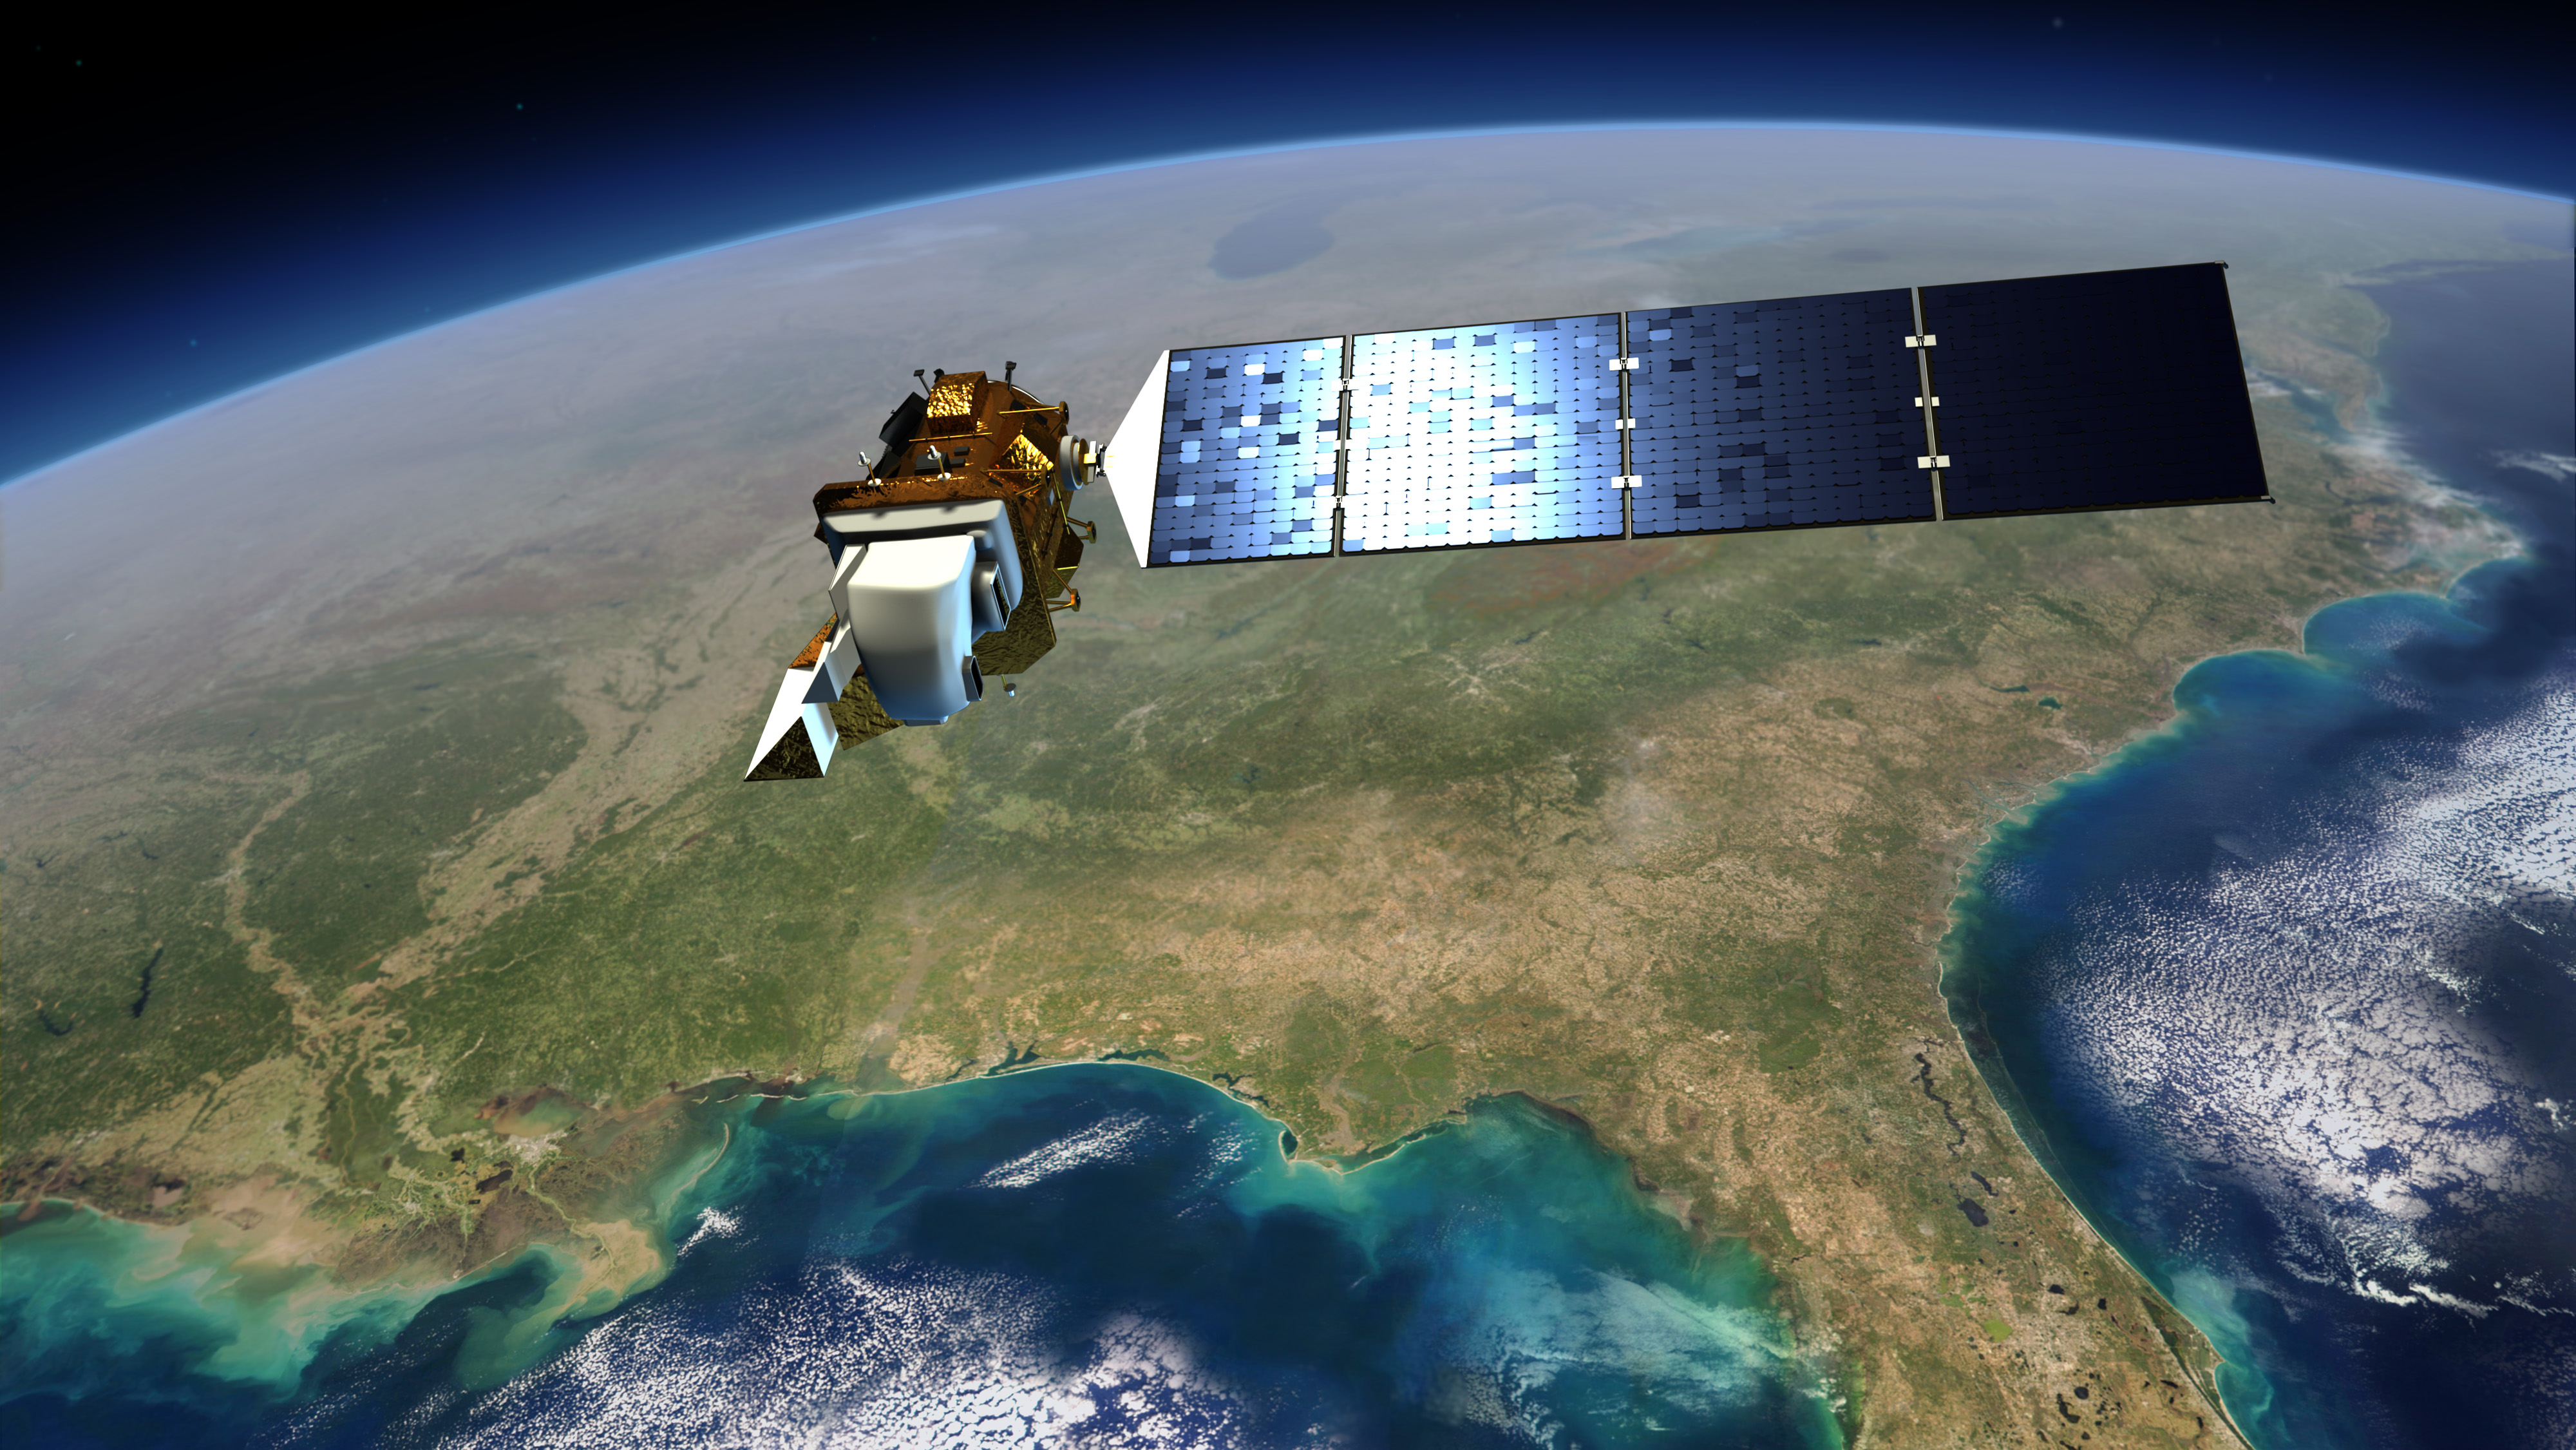
\includegraphics[width=0.6\textwidth]{01.1-introduction/figures/earth_satellite}
	};
	
	\end{tikzpicture}
	
	% source: https://code.earthengine.google.com/802d139566c47d63a7233109af117aba
\end{center}

\textbf{Keywords:} literature overview, datasets, multi-spectral satellite imagery, spectral water indices, outline

\end{abstract}


%% Start the actual chapter on a new page.
\newpage

\section{Introduction}

\dropcap{W}{ater} is one of the key sources of life on Earth, and it is constantly changing: waves batter the coast causing erosion, river banks are transformed under the flow of water, glaciers are melting, resulting in new lakes and wetlands, reservoirs and harbors are constructed, and much more. Accurate estimation of these surface water changes is crucial for a better understanding and management of the natural and anthropogenic processes causing them. 

For decades, satellites were used to accumulate large amounts of information, resulting in multi-petabyte archives of images collected. However, only during the last decade, due to recent developments in cloud computing,  we have started to transform these massive amounts of data into a valuable knowledge. The main limitations that were preventing analysis of these large archives of satellite data were their commercial nature. A breakthrough which enabled exploration of surface water at high spatial and temporal resolution was opening of access to Landsat mission data by NASA. It is only in 2008 that NASA has made Landsat 7 data freely available. Moreover, it took five more years to ensure that the first global-scale research results would be produced where these datasets could be explored to the full extent \citep{Hansen2013}.

% http://www.spacenewsmag.com/feature/the-state-of-the-satellite-industry-in-5-charts/

The number of satellites orbiting Earth is constantly increasing, as well as their technical characteristics, resulting in a better spatial, temporal, spectral, and radiometric resolutions. In the last years, the number of Earth Observation (EO) satellites launched to the Earth's orbit, and the number of observed images increased exponentially, mainly due to the reduction of the satellite sizes and costs required for their delivery to the orbit. This rise of the satellite industry defines new scientific challenges, demanding more efficient and robust methods to process massive amounts of data in even more compelling ways. With the technological and methodological developments, the focus of the surface water analysis shifts towards planetary-scale analysis, enabling development of a more objective understanding of the Earth's natural and anthropogenic processes. Until recently \citep{Hansen2013, pekel2016high}, such planetary scale monitoring and long-term estimates of land use change estimates at high spatial resolution estimates were not feasible. 

\section{Cloud computing - a new era for satellite image processing}

The massive growth in volumes of satellite data has resulted in a severe demand in storage, computation and smart analytics to enable analysis of planetary-scale data. Until recently, such analyses were performed by highly specialized scientists and engineers, and on a case-by-case basis. New cloud platforms for large satellite data analysis, such as Google Earth Engine \citep{Gorelick2012}, rapidly remove thresholds to use planetary-scale data. The initiative to provide free access to supercomputer power for non-for-profit organizations and researchers was first time mentioned in 2009\footnote{\url{http://blog.google.org/2009/12/seeing-forest-through-cloud.html}}, followed up by the official release of the platform in 2010\footnote{\url{http://blog.google.org/2010/12/introducing-google-earth-engine.html}}. This platform provides access to a plethora of satellite information in three ways: (1) storage of satellite data in the cloud; (2) provision of computational resources; and (3) availability of analytical tools to process data into a clear end product. Since then, it has resulted in numerous academic achievements, which have helped to analyze and better understand Earth's surface changes happening during the last few decades \citep{Hansen2013}, \citep{pekel2016high}.

\begin{figure}
	\centering
	\includegraphics[width=1\textwidth]{01.1-introduction/figures/scenes-per-year}
	\caption{The number of Landsat and Sentinel scenes measured during the last four decades and used in the analysis}
	\label{fig:sensor-count}
	% source: BigQuery https://bigquery.cloud.google.com/results/aqua-monitor:bquijob_70d5924c_15a6512603d
	% L5 back to life in 2012: https://code.earthengine.google.com/ab333594ecae50596fe28a8b773d9d60
\end{figure}

The datasets used in the current research account for more than 11 millions of freely available medium resolution images observed by LANDSAT, ASTER, Sentinel-1, and Sentinel-2 missions from National Aeronautics and Space Administration (NASA) and European Space Agency (ESA) during the last four decades. For several examples, images from HYPERION hyperspectral sensor from the EO-1 mission will be used, there are only about 86000 of HYPERION images available globally, acquired during the last fifteen years, but their spectral resolution is more than 20 times higher when compared to other sensors. The resolution of the sensors varies from 10-30m for optical and SAR bands, and 90-120m for thermal bands. The \ref{fig:sensor-count} shows the total number of multispectral and SAR scenes acquired by these sensors during the last decades. A total size of these datasets as for 2017 is almost 2 petabytes large. The analysis of this magnitude of dataset requires the use of large scale hardware and software infrastructures capable of processing it. Using calculation similar to \citep{wagner2015big}, it would take \textbf{two years} to download this dataset on 100Mbit/s network and then another \textbf{126 years} to process it from raw formats to Level 1 products on a single machine assuming 4Mbit/s processing speed.

\section{Multispectral satellite sensors and freely available data}

In a raw form, satellite images require the use of specialized algorithms, frequently adjusted to detect specific features, quantify land use changes, or identify anomalies. The main reasons why satellite data processing is difficult is that they mostly represent many natural and human-made processes. Frequently very dynamic and interfering with each other. The resulting observations are frequently limited by technical limitations of the sensors and data processing pipelines. The presence of clouds, aerosols, and complex topographic conditions, as well as technical sensor limitations, result in multiple types of noise or gaps in the measurements, which needs to be addressed before any valuable information can be extracted from the satellite data.

The present research focuses mainly on the use of multispectral satellite imagery. This includes 30m multispectral imagery measured using Thematic Mapper (TM) sensor, used for Landsat 4 and 5 missions, Enhanced Thematic Mapper Plus (ETM+) sensor, used for Landsat 7 mission, and Operational Land Imager (OLI) and Thermal Infrared Sensor (TIRS) sensors on board of Landsat 8. The spatial resolution of most of these sensors is 30m, including 15m for the panchromatic band and 90-120m for thermal sensors. For a part of research, the data measured by a new 10m resolution satellite from ESA, Sentinel 2A, launched in 2015, as well as 15m resolution imagery from ASTER mission \citep{REF} were used.  All of the sensors mentioned above are capable of measuring light in multiple spectral bands, comprising visible and infrared parts of the electromagnetic spectrum as shown in \ref{fig:sensor-bands}.

\begin{figure}
	\includegraphics[width=1.0\textwidth,left]{01.1-introduction/figures/bands}
	\caption{Spectral bands of the Landsat, ASTER, and Sentinel 2 satellite sensors. Atmospheric transmittance is estimated using the MODTRAN4 model as discussed in \citep{verhoef2003simulation}}
	\label{fig:sensor-bands}
\end{figure}

The processing of multispectral satellite imagery usually involves many steps, including geometric and radiometric calibration. As for Landsat and ASTER missions, the raw images represent uncalibrated radiance values for every spectral band, stored as at-sensor measured digital numbers ($DN_\lambda$), which need to be manually converted into top-of-atmosphere (TOA) spectral radiances ($L_\lambda$) and reflectances ($\rho_\lambda$). See \citep{chander2009summary} for details on the required steps. Generating spectral radiance values uses trivial linear equation formula:

\begin{samepage}
	\begin{equation}
	\label{eq:radiance}
	L_\lambda = \alpha_\lambda \times Q_\lambda + \beta_\lambda
	\end{equation}
	
	where
	\\
	
	$L_\lambda$ - spectral radiance at the sensor's aperture $[W/(m^2 \times sr \times \mu{m}]$
	
	$\alpha_\lambda$ - band-specific rescaling gain factor  $[W/(m^2 \times sr \times \mu{m} / DN]$
	
	$\beta_\lambda$ - band-specific rescaling bias factor  $[W/(m^2 \times sr \times \mu{m} / DN]$
	
	$Q_\lambda$ - quantized calibrated pixel value $[DN]$
	\\
\end{samepage}

For multi-temporal analysis, TOA reflectance needs to be calculated to compensate for image-to-image solar irradiance differences. These calculations can be done using the equation:

\begin{samepage}
	\begin{equation}
	\label{eq:reflectance}
	\rho_\lambda = \frac{\pi \times L_\lambda \times d^2}{ESUN_\lambda \times \cos \theta_s}
	\end{equation}
	
	where
	\\
	
	$\rho_\lambda$ - spectral reflectance, indicating amount of solar energy reflected from the Earth's surface
	
	$d$ - Earth-Sun distance in astronomical units $[AU]$
	
	$ESUN_\lambda$ - mean spectral solar irradiance $[W/(m^2 \times \mu{m}]$
	
	$\theta_s$ - solar zenith angle $[degrees]$
\end{samepage}
\\

In contrast to Landsat and ASTER, a more recent Global Monitoring for Environment and Security (GMES) initiative from the European Commission (EC) and ESA resulted in the launch of two Sentinel-2 satellites \citep{drusch2012sentinel}. The data products provided by these satellites already include steps shown by equations \eqref{eq:radiance} and \eqref{eq:reflectance} and represent TOA reflectances for 13 spectral bands. 

For higher level data products, additional steps may be performed, such as atmospheric corrections, usually required for a more accurate spectral analysis. Atmospheric correction allows compensating effects caused by aerosols, for more information see \citep{gao2006review}. Additional steps may involve topographic correction, where local effects of relief are corrected as well, such as \citep{Tan2013}.

If this study, if not mentioned otherwise, most of the analysis is based on the top-of-the-atmosphere (TOA) spectral reflectance values. As will be seen later, this provides a good compromise for water detection applications and allows the use of methods to combine products generated by different satellite missions.

\section{Methods of surface water detection from multispectral images}

Luckily, spectral signatures of water in most clear-sky observations are very distinctive and can be easily detected even when using only TOA data products, which are not corrected for atmospheric effects. 

However, limited spectral, spatial and radiometric resolution of the sensor and many other factors may significantly influence the accuracy of the detected surface water (\citep{Ji2009}).

Existing methods for surface water detection from multispectral satellite data use the fact that water significantly absorbs most radiation at near-infrared wavelengths and beyond. This fact makes it easy to detect clear water employing spectral indices, such as the Normalized Difference Water Index (NDWI), which can be interpreted simply as the slope of a spectral curve \citep{McFeeters1996}:

\begin{equation}
NDWI =  \frac{\rho_{green} - \rho_{nir}}{\rho_{green} + \rho_{nir}} 
\label{eq:index_NDWI}
\end{equation}

where $\rho_{green}$ and $\rho_{nir}$ correspond to the spectral reflectance of green and near-infrared bands. By design, the index (similarly to normalized difference vegetation index \citep{rouse1974monitoring}) values vary between -1 and 1, with water appearing mostly when the index value is greater than zero.

This index should not be confused with another one, also called NDWI and introduced by \citep{Gao1996} to detect water stressed vegetation. The Modified Normalized Difference Water Index (MNDWI) \citep{Xu2006}, appears to be more sensitive, due to the use of shortwave infrared band instead of the near-infrared in NDWI. The authors claim that the index results in a better surface water detection in urban areas when compared to the use of the near-infrared band. 

\begin{equation}
MNDWI =  \frac{\rho_{green} - \rho_{swir1}}{\rho_{green} + \rho_{swir1}} 
\end{equation}

While NDWI and MNDWI are among the most widely used spectral indices for water detection, many other efforts have been made trying to develop a new spectral index for surface water detection, based on a simple linear band combination AWEI (\citep{feyisa2014automated}), WI$_{2015}$ (\citep{fisher2016comparing}) and based on HSV transformation (\citep{pekel2014near}). An excellent overview and comparison of performance for some of these indices for Australia can be found in \citep{fisher2016comparing}. Even though the WI$_{2015}$ were reported to perform better than the classical NDWI index, the general conclusion of the authors was that each index was highly dependent on the composition of the validation pixels, and no index performed best across all water and non-water pixel types. The same paper mentions, that very little studies were done, comparing strengths and weaknesses of different spectral water indices. 

The detection of surface water from cloud-free images is simple, but doing this for noisy images is hard. Most of existing methods, when applied to the real-world satellite imagery, require manual tuning and, in general, need to be significantly adjusted to be used for planetary scale analysis. The task of surface water detection becomes much more challenging in the case of cloud, haze, snow or ice presence. 

\section{What are the main challenges of surface water detection?}

While water detection from cloud and snow free multispectral images appears to be trivial, it remains a very challenging task when working with the real world images. In this case, clouds, snow, and ice may frequently be misinterpreted as water. The land surface may be covered by snow for a significant time of the year, especially in temperate and cold climate zones. Additionally, errors of commission (false positive detection of water) can be observed in areas with shadows due to topographic conditions or presence of clouds. Recently (\citep{Zhu2014} and \citep{Zhu2012}), Zhu has introduced a set of methods for clouds, cloud shadows, and snow detection which are currently employed by NASA/USGS to process all Landsat images. To detect cloud shadows, these methods make use of information on satellite sensor view angle and solar zenith/azimuth and are also used to produce Surface Reflectance Landsat products \citep{webLandsat}. These parameters, combined with elevation data, can also be used to detect hill shadows \citep{Tan2013}. An alternative approach to exclude clouds and shadows is the use of average reflectance composites instead of instantaneous images \citep{Potapov2012}, \citep{Hansen2013}. However, this averaging usually damages spectral signatures of the surfaces, limiting the application of some methods, such as spectral unmixing \citep{keshava2003survey}.

\subsection{Variability of water spectral signatures due to natural and human-made processes}

One of the reasons why water classification from multispectral imagery is a very challenging task is that most of the observed surface water pixels are not noise-free. Mostly, it is a mixture of spectral signatures generated by a combination of different materials observed at a given time and location. Additional factors, resulting in spectral mixtures, are the physical limitation of the satellite sensors, such as spectral and spatiotemporal resolution, but also, systematic errors of the data processing pipeline. Many of the factors, influencing spectral signatures of observed water bodies, are caused by very non-stationary events, impossible to predict very accurately. Such as movement of clouds and aerosols in general, snow and ice cover changes, and suspended or diluted substances present in water. 

\begin{figure}
	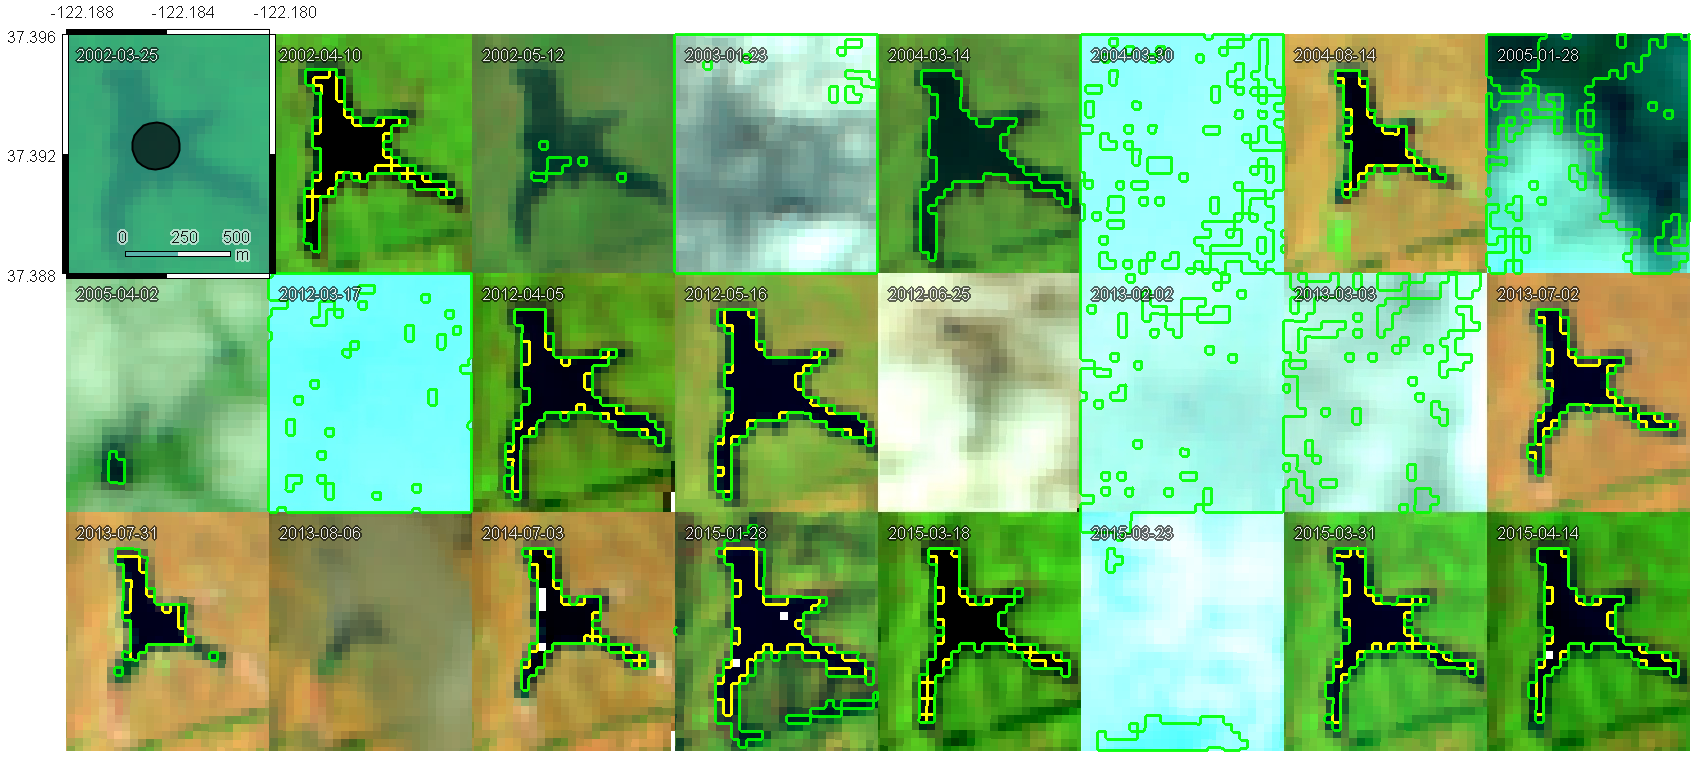
\includegraphics[width=1.0\textwidth,left]{01.1-introduction/figures/hyperion-map}
	\caption{Hyperion image mosaic for 2002-2015, showing the variability of land cover, seasonal vegetation changes and hill shadow processes over Felt Lake, USA, CA. Green and yellow edges indicate values of $NDWI=0$ computed using two band combinations: $\lambda_{b18, b54} = [528nm, 895nm]$ (green) and $\lambda_{b24, b50} = [589nm, 854nm]$ (yellow).
	Source: \url{https://code.earthengine.google.com/23048e43a9cf677d0b183224ecd1dac8}} 
	\label{fig:intro-hyperion-example}
	
\end{figure}

\begin{figure}
	\includegraphics[width=1.0\textwidth,left]{01.1-introduction/figures/hyperion-signatures}
	\caption{Hyperion spectral signatures measured at-sensor for the images on \ref{fig:intro-hyperion-example} sampled as a mean around waterbody center with a buffer of $r=90m$ radius. Most of the spectral signatures with the values $\rho_{\lambda = 400nm} < 0.2$ belong to water.} 
	\label{fig:intro-hyperion-example-signatures}
\end{figure}

Figure \ref{fig:intro-hyperion-example} shows a few examples of multispectral satellite images, in this case, measured by hyperspectral sensor Hyperion. For this specific area, about 50\% of the images are covered or partially covered by clouds, haze of fog. The green and yellow edges show where two variations of $NDWI$ index are equal to zero. It can be seen that default threshold fails to detect water boundary correctly in most examples. This happens mainly due to clouds, shadows, and mixed pixels types of noise present in the images. Additionally, significant differences can be observed between two indices constructed using slightly different band combination. A more detailed analysis of the reasons why this happens and different automated methods to overcome this problem will be discussed in Chapter \ref{ch2}.

Figure \ref{fig:intro-hyperion-example-signatures} shows the actual variability of spectral curves observed for this location, converted from DN numbers to radiance and subsequently, to reflectance values. Multiple interconnected events result in increasing complexity of the tasks aiming to recover the actual land use classes observed at a given location and time.

Automatic and accurate reconstruction of surface water from very noisy images is, in general, a tough task, and there is no method works perfectly for all land use types and atmospheric conditions. Most of the processes which occur in the same area and are observed by the satellite sensor are very random, with unknown distribution and are very hard to model using existing methods. However, some recent efforts in applying more advanced statistical learning methods, based on such as Bayesian Networks \citep{mello2013bayesian}, Conditional Random Fields \citep{hoberg2015conditional}, Markov Random Fields \citep{elmi2016dynamic}, and Deep Learning \citep{chen2014deep}, look very promising.

\subsection{Spectral and radiometric resolutions}

When working with multi-mission satellite data, the radiometric resolution is another factor which may influence surface water detection.  Radiometric resolution refers to the sensitivity of the sensor to incoming radiation, which is characterized by the minimum and maximum radiance values as well as the number of bits used to store measured values. Usually, this value varies between 8 and 16 bits. For Landsat TM, ETM+, and ASTER sensors the effective radiometric resolution is 8-bit. For Landsat 8 and Sentinel-2, it was improved to 12 bit (stored as 16 bit). For most of the applications, the effect of these subtle changes in radiance is neglected. However, the effect of 8-bit radiometric resolution may influence thresholds used to detect surface water, especially water is mostly represented in low radiance values.

\subsection{Spatial and temporal resolution}
For the sensors studied in the present research, the spatial resolution of the sensors varies between 10m to 30m for optical and SAR bands. For thermal bands, which were used mainly for cloud and snow masking, spatial resolution varies in the range of 60m-120m. 

\begin{figure}
	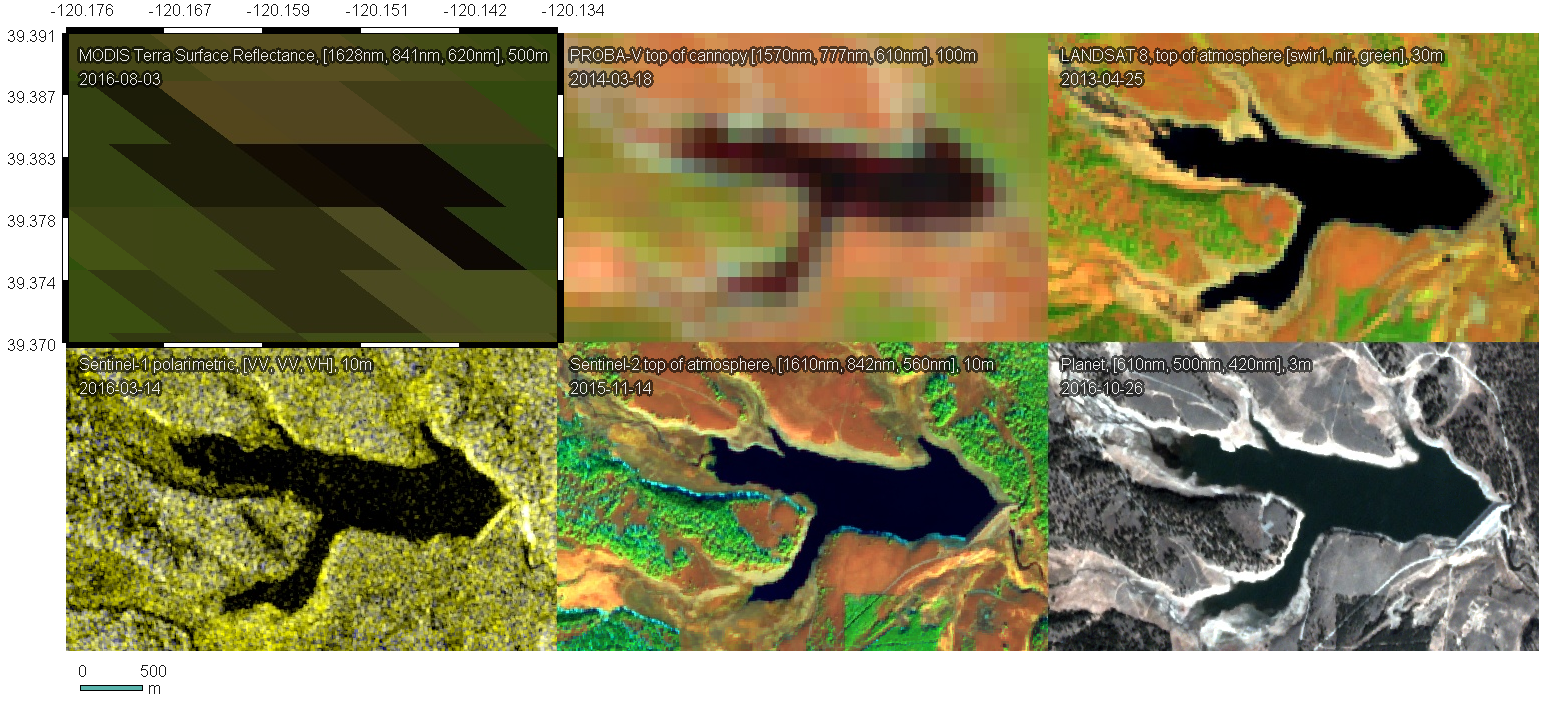
\includegraphics[width=1.0\textwidth,left]{01.1-introduction/figures/example-resolutions}
	\caption{Examples of images with different spatial resolutions, from six different multispectral sensors, Prosser Creek Reservoir, Nevada County, California, USA. Source: \url{https://code.earthengine.google.com/e09497a0f8cd6d20b1ce3b29600b958d}}
	\label{fig:example-resolutions}
\end{figure}

Figure \ref{fig:example-resolutions} shows a few examples of cloud-free satellite images over the same area. As can be seen, while medium (30m) to high resolution (3m) images can be used to resolve most of the reservoir boundary variations, it may become a challenging task to accurately estimate surface area using images with coarser resolution. Though, recent developments of more advanced super-resolution image processing techniques based on convolutional neural networks can be applied to reconstruct the actual shape of the water boundary using even very coarse and damaged representation \citep{ledig2016photo}, \citep{shi2016real}, \citep{johnson2016perceptual}. For remote sensing applications, a recent overview of different methods based on superresolution paradigm can be found in \citep{garzelli2016review}. The use of these methods goes beyond the scope of this thesis.

At the same time, temporal resolution mismatch between observations and the actual changes occurring on the land surface may significantly influence the applicability of satellite data for multi-temporal analysis. However, for some specific types of surface water changes, generative methods can be used to predict the actual state of waterbodies, by combining data from historical changes. One of these methods will be discussed in the Chapter \ref{ch3}, where a new generative algorithm will be developed to improve the estimation of surface water extent. This method is then applied to fill in water pixels which are missing, either due to the presence of noise, such as clouds or snow or due to a limited swath width of the satellite.

\subsection{Clouds and cloud shadows}

Detection and correction of effects caused by clouds and aerosols are probably the most studied topics of optical remote sensing. Clouds, haze, fog and other substances, cause absorption and scattering of the solar electromagnetic flux on its way to the Earth surface and then, on the way back to the satellite sensor. Many methods exist, providing atmospheric radiometric correction. The simplest approaches are easier to implement, such as dark-object subtraction (DOS) \citep{chavez1996image}, which is based on searching for the darkest object of the image and subtracting if from the radiances observed at-sensor. The drawback of this correction is that it may generate unrealistic results when the darkest pixels do not represent the actual dark object. More advanced methods involve simulation of the path radiances, using auxiliary data, such as information about aerosols \textbf{S}econd \textbf{S}imulation of a \textbf{S}atellite \textbf{S}ignal in the \textbf{S}olar \textbf{S}pectrum (6S) \citep{vermote1997second}, \citep{zhang2012improved} or \textbf{MOD}erate resolution atmospheric \textbf{TRAN}smission (MODTRAN) \citep{berk1987modtran}. 

Several satellite missions, such as Landsat, MODIS, and PROBA-V, already provide higher-level surface reflectance (SR) products, where images are corrected for atmospheric effects. Additionally, some of the data providers include quality assessment (QA) band, which indicates if the pixel is covered by clouds. However, the use of atmospherically corrected images from different satellite missions may result in a mismatch between images, even though the resulting images look more appealing and match better the ideal spectral signatures of different land cover types. At the time or writing this thesis, the official NASA/USGS Landsat SR products were still provisional. The documentation also mentions that the efficacy of SR correction is likely to be reduced in areas where atmospheric correction is affected by adverse conditions\footnote{Google Earth Engine Landsat 5 SR Dataset: \url{https://code.earthengine.google.com/dataset/LANDSAT/LT5\_SR}}:

\begin{enumerate*}[label=(\emph{\alph*})]
	\item SR is not run for a scene with a solar zenith angle greater than 76°
	\item SR quality reduces for data acquired over high latitudes (> 65°)
	\item The panchromatic band is not processed to SR
	\item Hyper-arid or snow-covered regions
	\item Low sun angle conditions
	\item Coastal regions where land area is small when compared to adjacent surface water
	\item Areas with extensive cloud contamination
\end{enumerate*}

Furthermore, There are issues with artifacts in the data over certain geographic areas, specifically: inland water bodies, areas of high relief, and areas with high aerosol abundance. 

\begin{figure}
	\includegraphics[width=1.0\textwidth,left]{01.1-introduction/figures/sr-RGB}
	\caption{Top of the atmosphere reflectance (left) and surface reflectance (right) false-color composite image (swir1, nir, green). Source: \url{https://code.earthengine.google.com/e09497a0f8cd6d20b1ce3b29600b958d}}
	\label{fig:example-sr-rgb}
\end{figure}

\begin{figure}
	\includegraphics[width=1.0\textwidth,left]{01.1-introduction/figures/sr-SNG}
	\caption{Top of the atmosphere reflectance (left) and surface reflectance (right) true-color composite image. Source: \url{https://code.earthengine.google.com/e09497a0f8cd6d20b1ce3b29600b958d}}
	\label{fig:example-sr-sng}
\end{figure}

The above issues with SR Landsat products, as well as the inconsistency between different SR methods used for different satellite products (Sentinel-2, Landsat) as well as missing SR products for some sensor (ASTER, EO-1) resulted in that this study mostly focuses on the use of TOA reflectance images. The main reason is that most of the higher level products use different atmospheric correction algorithms, which does not necessarily lead to improved classification. Additionally, for single-image based classification of surface water using adaptive methods, based on maximum likelihood principle, this type of correction may not be required \citep{song2001classification}.

It is important to note that for water detection the use of TOA can be even preferable, especially, when working with multi-mission satellite products. The main reason for this is that the auxiliary datasets used to generate SR products are usually of a coarser spatial resolution, which may introduce additional error to the image, even though the resulting spectral signal may be better. 

We will show, that even without SR correction, the TOA images can be used to detect surface water very accurately when automated methods of dynamic thresholding are applied. Additionally, the use of SR products for surface water detection may not be required when working with multi-spectral satellite imagery, because most of existing methods of surface water detection may use of near-infrared and infrared bands, which are less sensitive to aerosols. The effect of SR correction is much more evident for the visible part of the spectrum (Figure \ref{fig:example-sr-rgb}) when compared to false-color composite using infrared and near-infrared bands \ref{fig:example-sr-sng}.

Even though existing methods of SR correction can significantly improve radiometric properties, most of the methods are based on a single image only (ACCA, \citep{irish2006characterization}), which assumes, that significant amount of aerosols remain uncorrected, as well as secondary effects, such as cloud shadows. 

One of the recent advancements in single-image cloud and projected cloud shadow detection is FMask\footnote{FMask algorithm source code: \url{https://github.com/prs021/fmask}}, \citep{zhu2012object, zhu2015improvement}. The method was so successful that it is currently used to reprocess all Landsat images acquired. 

To fully eliminate the influence of clouds and cloud shadows, more advanced methods are required, focusing on \begin{enumerate*}[label=(\emph{\alph*})]
	\item detection of the pixels partially or completely damaged by atmospheric artifacts
	\item filling of missing pixels using methods of statistical inference
\end{enumerate*}. 

The FMask algorithm also provides surface water as a side product. However, the accuracy of the resulting water mask can be very inaccurate, especially, when dealing with mixed pixels, where images are only partially covered by cloud cover, as shown in figure \ref{fig:cfmask}.

\begin{figure}[H]
	\includegraphics[width=1.0\textwidth,left]{01.1-introduction/figures/cfmask}
	\caption{(\textcolor{red}{red}), cloud shadows (\textcolor{yellow}{yellow}) and surface water mask (\textcolor{blue}{blue}) as detected by FMask algorithm. Source: \url{https://code.earthengine.google.com/b74dc921e6725cffd1b29bca5b6d3c43}}
	\label{fig:cfmask}
\end{figure}

Some of the recent enhancements of the methods include the use of multi-temporal methods to further improve the accuracy of cloud and cloud shadow detection methods, TMask\footnote{TMask algorithm source code: \url{https://github.com/prs021/tmask-algorithm}}, \citep{zhu2014automated}. The main idea of the method is to extend the multi-step FMask algorithm by a new step, where a harmonic model is used to simulate the most probable reflectance values. The method is based on the seasonal changes of the reflectance values for pixels covered by vegetation. However, the authors mention, that the method may falsely identify ephemeral pixels as clouds or cloud shadows. To our experience, the applicability of the method is limited to areas with significant surface water dynamics. Additionally, the authors mention that the method performs extremely slow, making it nearly impossible to scale for global analysis, where millions of satellite images need to be processed. We will discuss in Chapter \ref{ch3} how probabilistic models can be used to identify clouds and cloud shadows as an alternative to this approach. 

A comprehensive study on the cloud cover variability has been performed recently by \citep{wilson2016remotely}\footnote{\url{http://www.earthenv.org/cloud}}. Even though the study focuses on a 1km spatial resolution only, it provides detailed intra- and inter-annual analysis of cloud cover frequency. These parameters can be crucial when developing data-driven models for cloud mask and cloud shadow detection. However, methods of high-resolution cloud and cloud shadow detection are still being actively developed, and no universal method exists yet which can provide an automated way to detect clouds and cloud shadows at high spatial resolution. 

\subsection{Snow and ice}

Snow and ice can cover a significant area of waterbodies in temperate and cold climates and need to be detected accurately to prevent misinterpretation of detected surface water. In general, snow/ice can be easily detected. In the first place, using the thermal band (most of the water bodies usually freeze at zero degree Celsius under normal conditions).  Additionally, methods of snow and cloud detection have been studied for a long time using a normalized difference snow index (NDSI), \citep{valovcin1976snow}, \citep{hall1995development}, defined as:

\begin{equation}
NDSI=\frac{\rho_{green}-\rho_{swir}}{\rho_{green}+\rho_{swir}}
\end{equation}

where swir and green bands correspond to wavelengths of $\lambda_{green}=~660nm$, $\lambda_{swir}=~1600nm$. It must be noted, that the MDNWI spectral index in \ref{eq:au_MNDWI} exactly repeats the definition of NDSI index. This fact makes it more difficult to discriminate water from snow when using MNDWI index. In general, a good separation still can be achieved by involving near-infrared as well, which is less sensitive to snow/ice content.

\begin{figure}[H]
	\includegraphics[width=1.0\textwidth,left]{01.1-introduction/figures/NDWI-NDSI}
	\caption{An example of Landsat 5 image for December 17, 2000 TOA composite image (left: swir1, nir, green) demonstrating how NDSI / MNDWI and NDWI spectral index values vary over snow-covered waterbody. Source: \url{https://code.earthengine.google.com/3b5de713c26202cad46e5ddfc5deb7c2}}
	\label{fig:snow}
\end{figure}

As can be seen in \ref{fig:snow}, it NDWI spectral index provides a more reliable way to discriminate between surface water and land pixels when snow and ice are present. This significantly limits the applicability of MNDWI spectral index, only to the multispectral images measured for warm year seasons, or to temporal composite images where snow cover is eliminated.

\subsection{Topographic effects}

Topographic illumination effects (hill or building shadows) may significantly disturb the signal measured by satellite sensors, causing false-positive surface water detection. Additional illumination correction (known as the topographic correction) is required to compensate these effects. Illumination effects can be corrected by compensating for solar radiance due to topographic effects, usually described by Bidirectional Reflectance Disturbance Function (BRDF), which defines how light is reflected at the surface. In remote sensing, simplified formulas were introduced to compensate topographic effects for Lambertian and non-Lambertian surfaces. Some of the most known are cosine model, C correction models \citep{teillet1982slope}. Some other models were developed later, such as Minnaert, and SCS+C \citep{smith1980lambertian, teillet1982slope}. A good overview of some of the method can be found in \citep{gao2009simple, soenen2005scs+}. 

Most of the topographic correction models are based on the use of relative solar incidence angle, or illumination conditions, defined as:

\begin{equation}
\label{eq:ic}
IC = \cos(\theta) \cos(\alpha) + \sin(\theta) \sin(\alpha) \cos(\phi_{\theta} - \phi_{\alpha})
\end{equation}

where $\theta$ is the solar zenith angle, $\alpha$ is the topographic slope angle (0 = horizontal), $\phi_{\theta}$ is the solar azimuth angle, and $\phi_{\alpha}$ is the aspect angle of the topographic surface (0 = north). The resulting illumination variable $IC$ varies between -1 and 1. The simplest topographic correction methods assume that the surface is Lambertian (ideal surface, diffusely reflects light in all directions, isotropic). The cosine model normalizes the reflectance of any pixel based on the assumption that the total irradiance received at a given location is directly proportional to the cosine of the incidence angle ($i$ - the angle between the normal to the pixel surface and the solar zenith direction) \citep{teillet1982slope}:

\begin{equation}
\label{eq:cosine}
L_n = L \frac{cos(\theta)}{IC}
\end{equation}

where $L_n$ is the corrected reflectance and $L$ if the observed reflectance on the inclined surface. The cosine model assumes that the surface is Lambertian and is independent of wavelength. Further development of topographic correction algorithms resulted in the introduction of more advanced, semi-empirical models, such as C correction \citep{teillet1982slope}. A variation of empirical C model was then introduced by \citep{tan2013improved}, which assumes non-Lambertian surfaces and is based on empirical rotation in reflectance/illumination space. In topographically complex areas, the use of this model can significantly reduce commission errors in surface water detection applications. To demonstrate the effects of the topographic correction on the surface water detection, an empirical rotation model developed by \citep{tan2013improved} is applied to process Landsat image focused on the reservoir located in the mountain region (figures \ref{fig:ch1-topo-map} and \ref{fig:ch1-topo-chart}). 

\begin{equation}
\label{eq:topo-c}
L_n(\lambda) = L(\lambda) \frac{cos(\theta) + C(\lambda)}{IC + C(\lambda)}
\end{equation}

where ${\lambda}$ is a band-specific wavelength and the variable $C = b / a$ is an empirical coefficient equal to the ratio of slope $a$ and intercept $b$ of a linear regression performed for between reflectance and illumination conditions images:

\begin{equation}
\label{eq:topo-c-regression}
L(\lambda) = a(\lambda) \cdot IC + b(\lambda)
\end{equation}

To demonstrate results of the application of this model, we have applied it to correct satellite images in hilly area around a small reservoir in California, USA, Lake Piru.

The results of the topographic correction can be seen in figure \ref{fig:ch1-topo-map}, and corrected reflectance values for the near-infrared band are shown in figure \ref{fig:ch1-topo-chart}. As we can see, the topographic correction step significantly corrects original reflectance values. The correction was performed with the help of 3m National Elevation Dataset (NED) \cite{gesch2002national}.

\begin{figure}[H]
	\includegraphics[width=1.0\textwidth,left]{01.1-introduction/figures/topo-map}
	\caption{An example of topographic correction algorithm \cite{tan2013improved} applied to Landsat 8 false-color composite image (swir1, nir, green) acquired on November 5, 2013. Original image (A), corrected image (B), hillshade of NED DEM (C), NDWI computed from the uncorrected image (D), and NDWI computed from corrected reflectances (E). Dark circle indicates pixels used to produce the chart in figure \ref{fig:ch1-topo-chart}.  Source: \url{https://code.earthengine.google.com/90a3782edde7c0ef5ca895c800c1a688}}
	\label{fig:ch1-topo-map}
\end{figure}


\begin{figure}[H]
	\includegraphics[width=1.0\textwidth,left]{01.1-introduction/figures/topo-chart}
	\caption{Original (left) and corrected (right) values or near-infrared band aggregated over the marked circle area in \protect \ref{fig:ch1-topo-map}}
	\label{fig:ch1-topo-chart}
\end{figure}


The above model provides a much better correction of multispectral images. However, the corrected image may still contain small artifacts, caused by errors in elevation model and more complex light interactions. It is important to note, that topographic correction may need to be avoided if a significant variability of surface water mask between images takes place. In this cases, topographic correction may introduce local artifacts for the pixels where a mismatch occurs between digital elevation model and surface water edge.

For surface water detection, an alternative method is to exclude pixels where the topographic correction may be required. One way to perform this kind of masking is using Height Above the Nearest Drainage (HAND) topographic index \cite{Renno2008, Nobre2011}. HAND was used in multiple water detection studies using synthetic aperture radar (SAR) imagery \citep{Eilander2014}, \ref{amitrano2014sentinel}. 

% The use of InSAR with Sentinel-1 Single Look Complex (SLC) data to reconstruct digital surface model (DSM) around reservoir during dry seasons \ref{amitrano2014sentinel}.

Even though this method was almost not applied, it can be utilized to generate high frequency surface water mask in hilly areas in addition to the methods discussed in chapters \ref{ch2}, \ref{ch3} and \ref{ch4}. As an alternative, in Chapter \ref{ch6} we will use HAND to mask out errors in hilly areas for a global surface water change detection study. Additionally, HAND is utilized in the Chapter \ref{ch7} to identify hilly areas where additional unsupervised classification step is required to refine surface water mask.

\begin{wrapfigure}{r}{0.5\textwidth}
	\begin{center}
		\includegraphics[width=0.48\textwidth]{01.1-introduction/figures/Lake-Piru}
	\end{center}
	\caption{Lake Piru, California, USA. \protect \footnotemark}
\end{wrapfigure}

\footnotetext{Source: Flickr, \url{http://www.flickr.com/photos/tomsaint/3281932913}}

Even though topographic correction algorithms may significantly improve the overall image illumination for hilly areas, they may also introduce local artifacts when detecting surface water. The main reason is that the digital elevation models are mostly measured at a specific time only, but the actual water body boundary may vary a lot for ephemeral water. To avoid these errors, additional steps are required, for example as it will be described in Chapter \ref{ch3}, where density-based methods will be used to infer the actual water mask.

In some cases, it is possible to avoid topographic correction step, for example, when analyzing surface water changes using multi-temporal composite images, based on a large number of observations. However this is only possible under the assumption that the images are generated using image collections where illumination parameters (sun elevation and azimuth) are equally distributed, this will be discussed in more details in Chapter \ref{ch4} and \ref{ch6}.

% The figures \ref{fig:intro-topo-3-water}, \ref{fig:intro-topo-4-water-corrected} demonstrate results of surface water detection method in hilly areas without and with the topographic corrections applied.

\section{Global static and dynamic surface water datasets}
Global-scale surface water and its dynamics have been very actively studied in the last years; this includes estimation of both static surface water masks, such as 250m SWBD \citep{farr2007shuttle} and MOD44W \citep{carroll2009new}, as well as 30m GLCF \citep{feng2016global} and 90m G3WBM \citep{yamazaki2015development}. An overview and comparison of some of these datasets can be found in \citep{lamarche2017compilation}. Advances in the big data technologies and massive growth of the available satellite data have resulted in the appearance of new high-resolution datasets, with a significant increase in both temporal (from static to monthly) and spatial resolutions (30m) \citep{pekel2016high}. An overview of some of the static and dynamic surface water produces can be found in \citep{yamazaki2016hydrology}. 

The upcoming SWOT mission (2021) promises to deliver twice every two weeks monitoring of 90\% of global water bodies smaller than 100m. However, this will not answer the question about how surface water was changing during the last four decades. Moreover, the accurate knowledge of historical surface water dynamics is very important to fill in gaps in the trending hyper-resolution hydrological activities \citep{bierkens2015hyper}. A good overview of the recent advances and trends related to satellite-based EO for hydrology, in general, can be found in \citep{mccabe2017future}.

In addition to optical and radar surface water mapping, numerous studies were performed focusing on the reconstruction of surface water elevation changes using satellite altimetry: HydroWeb \footnote{HydroWeb: \url{http://www.legos.obs-mip.fr/soa/hydrologie/hydroweb/}} \citep{cretaux2005satellite}, DAHITI \footnote{DAHITI: \url{http://dahiti.dgfi.tum.de/en/}} \citep{schwatke2015dahiti}, G-REALM \footnote{G-REALM: \url{https://www.pecad.fas.usda.gov/cropexplorer/global_reservoir/}} \citep{birkett2011research}, HydroSAT \footnote{HydroSat: \url{http://hydrosat.gis.uni-stuttgart.de/}}. 

Recently, multiple global studies were performed where a hybrid approach was implemented to reconstruct reservoir and lake storage dynamics from satellite altimetry combined with optical multispectral satellite data \citep{khandelwal2016approach}, GRanD Viewer \footnote{GRanD Viewer: \url{http://umnlcc.cs.umn.edu/GrandViewer/}}. An overview of some methods to monitor large lakes and reservoirs as well as some challenges can be found in \citep{karpatne2016global}. Integration of the data on both water level and surface area changes can be used to generate high-resolution storage changes \cite{duan2013estimating}. In many cases, having only surface water extent changes should be sufficient for the reconstruction of the waterbody storage dynamics \citep{liebe2005estimation}. However, for accurate estimates of water storage dynamics, relations between volume and area need to be estimated very accurately.  Some of the recently developed methods include estimation of reservoir bathymetry from SAR data, through InSAR algorithms \citep{amitrano2014sentinel} or by estimating volume/area curves based on a topographic similarity \citep{bemmelen2016determining}. Estimating area/volume curves is currently one of the gaps to be filled using EO methods. This information is crucial for improving the local relevance of global hydrological studies. 

\section{Earth Observations (EO) and Volunteered Geographic Information (VGI)}
Many global surface water mapping efforts rely on the information derived from EO datasets, such as optical multispectral imagery, synthetic-aperture radar (SAR) imagery or radar altimetry. A combination of remote sensing with existing GIS vector data sets that contain information on water occurrence gets much less attention. GIS vector data sets are frequently measured using high-resolution GPS devices or by manually digitizing aerial or satellite imagery. As a result, these data sets usually demonstrate much better precision and contain semantic information, such as feature names, types, and other attributes. Their quality and completeness are not uniform around the globe. One key global vector data set containing water information is OpenStreetMap (OSM) \citep{Haklay2010}, initiated in 2004 and currently including more than 3 billion objects. From these, more than 8 million objects relate to water \citep{webOSMTagInfo}. Many environmental applications use OSM, including the extraction of paved area and surface water coverage for hydrological applications \citep{Schellekens2014}. 

The volunteered nature of OSM is the main factor that makes it less adopted by GIS professionals \citep{Mooney2010} stressing the importance of the development of automated methods and tools to validate its quality in comparison to other datasets. A good example of how OSM quality can be assessed can be found in \citep{Girres2010}, showing how positional differences between linear and polygonal features can be addressed. Furthermore, the “increasing buffer” method, \citep{Goodchild1997} can be used to estimate the quality of linear features. An excellent overview of papers focusing on OSM quality can be found in \citep{Barron2014}. The latter also suggests using elements of ISO 19113:2002 \citep{iso2002} (such as completeness, an error of commission/omission or positional differences) to evaluate the OSM quality. Unfortunately, to our knowledge, no academic literature exists focusing solely on the quality of water features present in OSM and using global or nearly global remote sensing datasets. 

In Chapter \ref{ch7}, we will compare surface water masks derived from OSM to see if it can be used as a complementary dataset to generate global coverage, even though its local coverage and quality may vary. 

\subsection{Reservoirs and their storage dynamics}
Even though many of the global waterbodies may change over time, most of the existing surface water vector maps are static, not providing any information on temporal spans where these features are valid. However, many of these vector datasets are incomplete in term of spatial coverage. On the other hand, satellite data provide a way to extract spatiotemporal variability of these waterbodies with a constantly increasing resolution. However, a very relevant information missing in the satellite-based products and available in vector topographic maps is semantics. This includes many attributes, such as names of the waterbodies, construction date, administrative information and much more. Some of these attributes, like construction time or surface area variability, can be extracted from satellite data. Others, like names, technical characteristics, need to be collected manually. At present, a hybrid approach to generate the best quality surface water maps seems to be the most promising, combining multi-temporal satellite information with existing vector maps, but also, results from numerical models, to estimate the variability of water-related parameters.

A lot of effort has been made trying to map water bodies at a global scale. However, existing databases are still scarce and fragmented, as can be seen in Figure \ref{fig:global-dams}\footnote{\url{http://bit.ly/global-dam-locations}}. Here we show location of reservoirs collected by different databases, including 6859 reservoirs and lakes in GRaND \citep{Lehner2011}, 4668 dams collected on Wikipedia\footnote{\url{https://en.wikipedia.org/wiki/Wikipedia:WikiProject_Dams}}, more than 150000 reservoir and dam locations available in OpenStreetMap \citep{webOSMTagInfo}, and 33684 global dams collected by King's College London \citep{mulligan2009global}. 

Detailed data on storage changes for many of these reservoirs is still incomplete but is required for an automated setup (generation and calibration) of surface and subsurface water models, essential to optimize water management use and to answer the upcoming challenges related to floods and water stress in the $21^{st}$ century \citep{hirabayashi2013global}.

\begin{figure}[ht]
	\begin{adjustbox}{addcode={\begin{minipage}{\width}}{\caption{
						Mapping of about 150000 global dam locations from multiple databases		
						}\label{fig:global-dams}\end{minipage}},rotate=90,center}
		\includegraphics[width=1.0\textheight]{01.1-introduction/figures/global-dams}
	\end{adjustbox}	
\end{figure}

Most of existing reservoir dataset are still incomplete, either regarding quality or coverage, resulting in that existing global hydrological models, (GLOFISS and GloFAS) still make use only coarse databases like GRaND, missing many small to medium size reservoirs \cite{emerton2016continental}.  Hence, the introduction of parallel processing platforms such as GEE and freely available access to higher resolution data such as Sentinel-2 open new possibilities to improve these datasets and to reconstruct historical surface water dynamics. The actual number of currently mapped small reservoirs and lakes is still unknown, as well as their surface area extent and storage variability.

\section{Conclusions}

Many artifacts present in satellite images require the use of a multi-step approach when the actual signal needs to be filtered from the noise, usually present in almost every satellite image.

Remote Sensing (RS), in general, and Earth Observation (EO) in particular is a rapidly growing field. During the last decade, it has resulted in an enormous amount of new datasets, with many datasets freely available. The amount of free data available is more than can be digested by the research community on a short term, so many multidisciplinary research questions, on both technological and algorithmic sides, remain open. 

One of the largest challenges is related to harmonization of the satellite data, simplifying processing to extract valuable information from multiple satellite data products, resulting in a higher temporal resolution. Luckily, this issue was also addressed by Google resulting in a parallel satellite data processing platform, solving many of the technical issues.

Simultaneously with the remote sensing datasets, many other high-resolution Earth-scale datasets become available. One of the fast-growing datasets is OpenStreetMap, but in general - any other georeferenced dataset. The main advantage of these type of dataset is the presence of semantic information (river names, administrative areas, property values and so on). This kind of information becomes crucial in performing higher-level studies, focusing on the impact assessment of short or long-term events which can be observed from space. Integration, but also cross-validation of the datasets with different origin will be crucial to maximize the value of these datasets and to improve their overall quality.

Technological developments and outreach efforts undertaken by large companies such as Google have resulted in the development of parallel processing platforms like Google Earth Engine. This platform has truly revolutionized processing of satellite imagery and has already led to a significant number of successful research efforts which could be unimaginable to perform otherwise, because of large amounts of data to be stored and processed.

While many methods exist to process multispectral passive sensor satellite imagery, the methods listed in this chapter are in my opinion the first to try when processing optical satellite imagery addressing surface water detection. 

For surface water detection, the use of surface reflectance imagery will not necessarily result in a better quality water masks, while the process of most high-quality surface reflectance products is very complicated. 

With the growing amounts of data, the need for automated methods for surface water detection from satellite images is higher than ever. One of the primary goals of this research was to develop a set of fully automated algorithms and software tools to enable processing of multi-spectral satellite imagery for surface water detection at high spatial and temporal resolutions. In the next three chapters \ref{ch2}, \ref{ch3} and \ref{ch4}, more advanced unsupervised methods will be introduced to address this. Examples of their applications are also included. 

For long-term as well as for permanent surface water detection studies (Chapter \ref{6} and \ref{ch7}), the use of composite images may be sufficient, while for other - the highest temporal and spatial resolution data may be required. For example, to study rapid surface water changes, such as floods, where the temporal resolution of physical processes is high and may require processing of all possible data sources to quantify the actual surface water dynamics.

